\documentclass[../main.tex]{subfiles}
\begin{document}

\chapter{Energilagring } \label{Chap:Energilagring}
Som energilager benyttes der en 1F superkondensator med maksimal spænding på 8.1V. Dette er helt fint, da vi ikke kommer til at overstige 5V. Superkondensatorens energilager sørger for at udglatte når energikilden skifter, så der altid leveres en stabil spænding og strøm til forbrugeren. Derudover fungerer den også som et batteri, og kan holde på spændingen hvis forbrugeren fjernes. Der er dog en del tab i de andre komponenter, så den holder ikke denne spænding længe, hvis der ikke bliver tilført noget energi fra kilderne.

\section{Test}
Krav 7 i kravspecifikationen siger at spændingen V3 skal være indenfor 5v +/- 0.5 volt ved strømme større end 20 mA. Dette opfyldes ved at belaste udgangen af energilageret med 66 $\Omega$ og måle spændingen. Figur \ref{fig: Krav 7 Opfyldt} viser at kravet er overholdt.

\begin{figure}[H]
      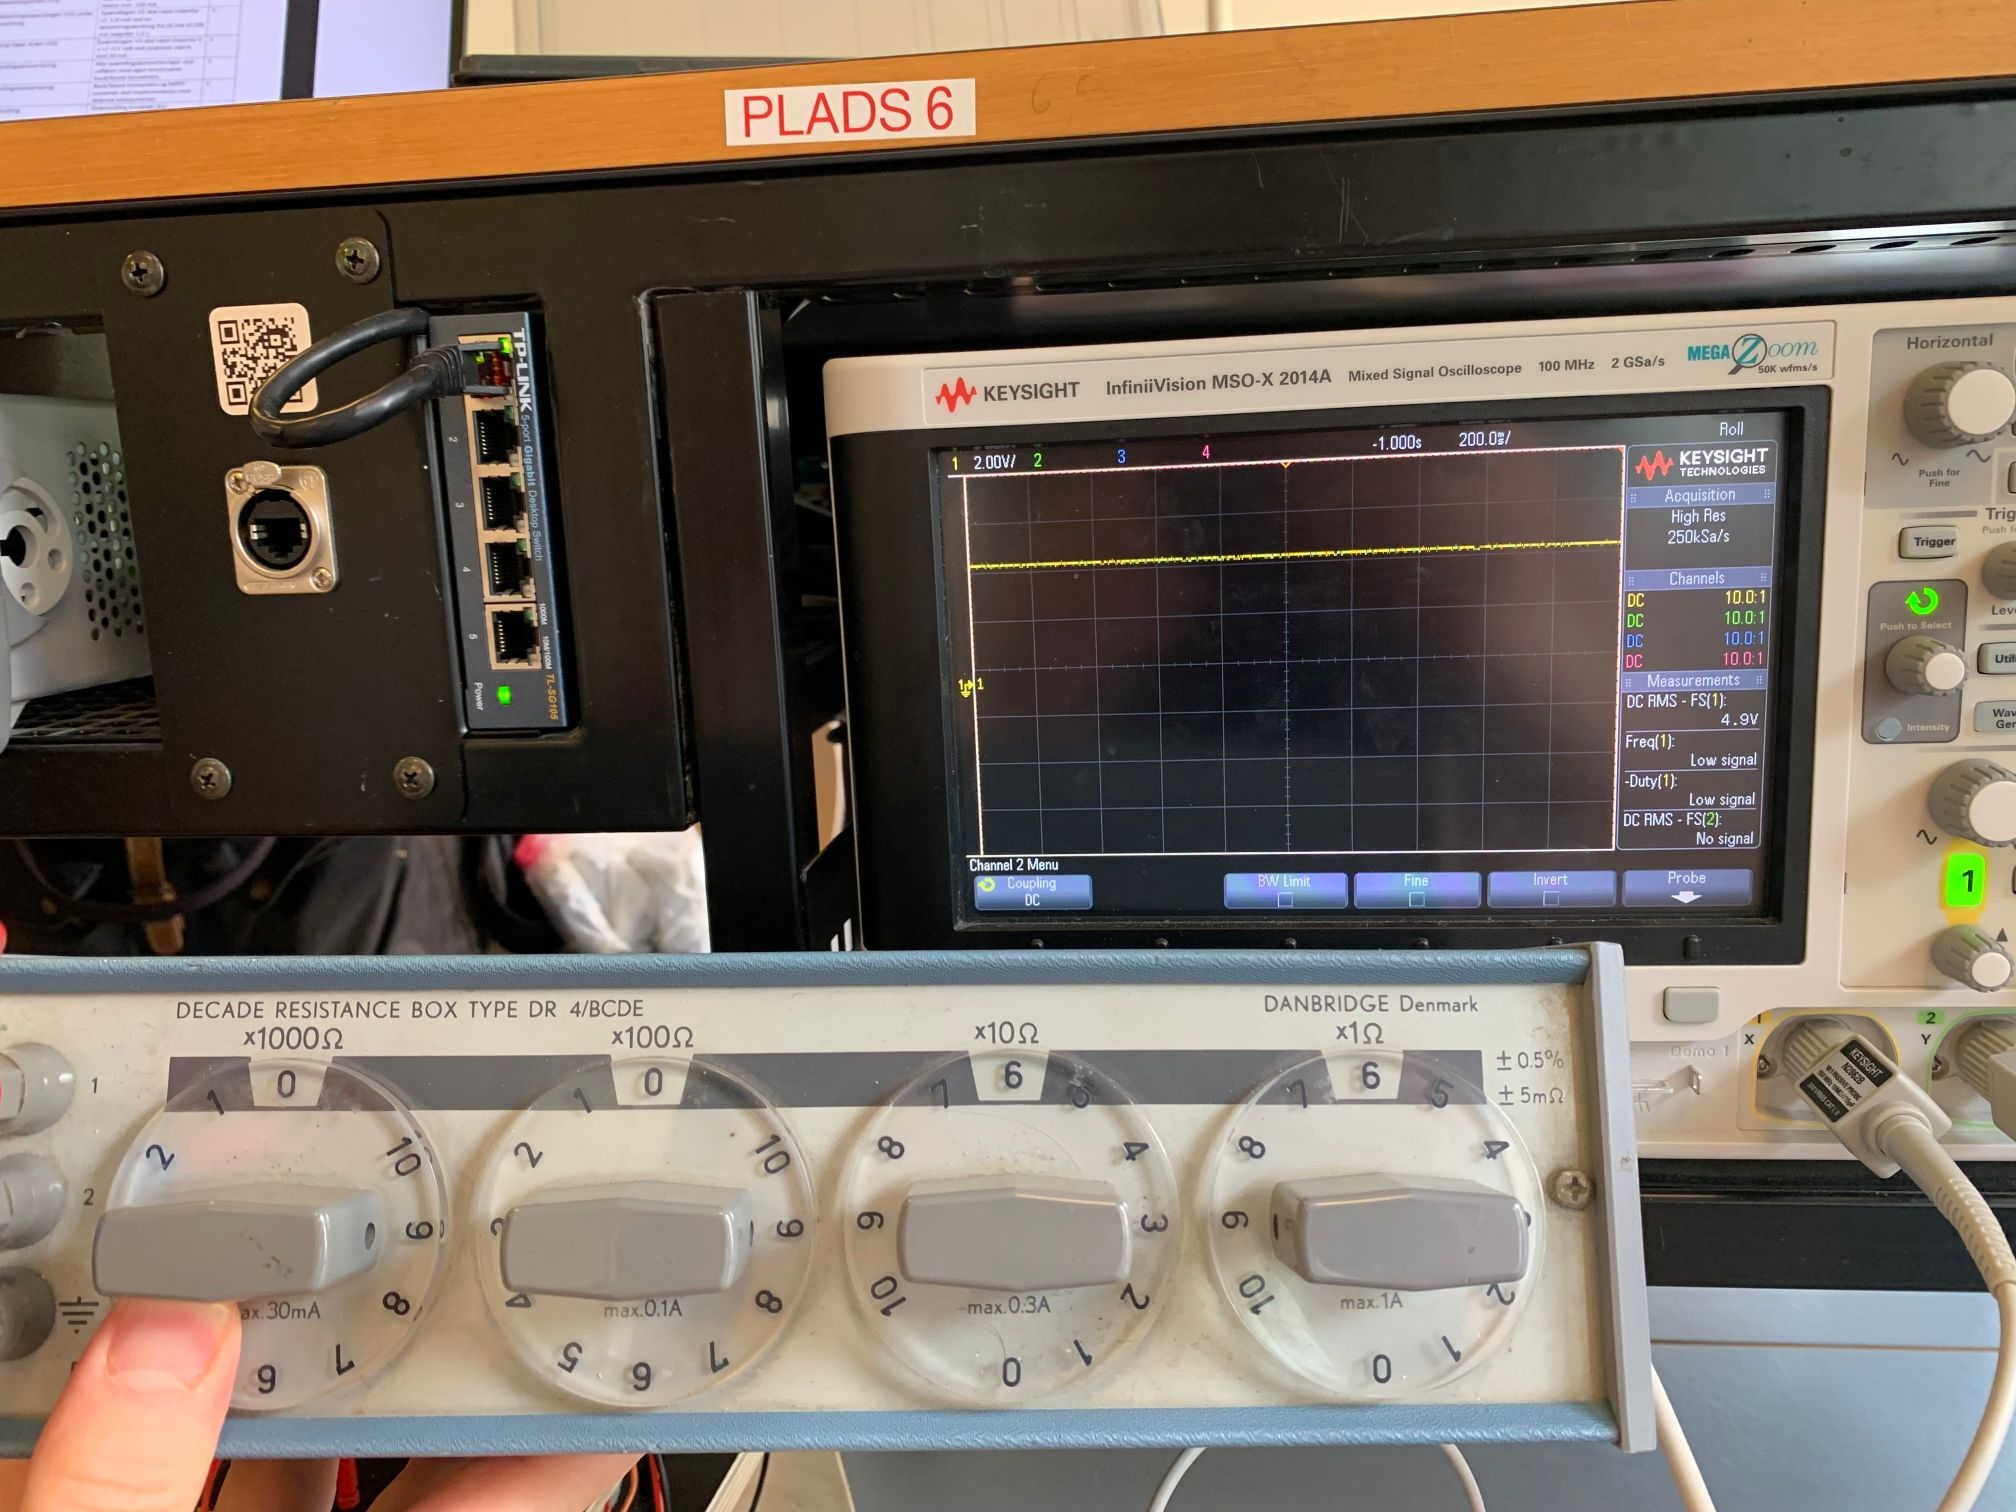
\includegraphics[width=\textwidth]{Dokumentation/Pictures/Krav7.jpg}
     \caption{Krav 7 Opfyldt}
     \label{fig: Krav 7 Opfyldt}
     \end{figure}


\end{document}

